\documentclass[sigconf]{acmart}

\usepackage{pgfplots}
\usepackage[utf8]{inputenc}
\usepackage{xcolor}
\usepackage{multirow}
\usepackage{hyperref}
\usepackage{listings}

\pgfplotsset{compat=1.8}
\usepgfplotslibrary{statistics}

\lstset{
language=C,
basicstyle=\scriptsize\ttfamily,
commentstyle=\ttfamily\color{gray},
numbers=left,
numberstyle=\ttfamily\color{gray}\footnotesize,
stepnumber=1,
numbersep=5pt,
backgroundcolor=\color{white},
showspaces=false,
showstringspaces=false,
showtabs=false,
frame=single,
tabsize=2,
captionpos=b,
breaklines=true,
breakatwhitespace=false,
title=\lstname,
escapeinside={},
keywordstyle={},
morekeywords={}
}


\setcopyright{none}
\settopmatter{printacmref=false}

%%%% As of March 2017, [siggraph] is no longer used. Please use sigconf (above) for SIGGRAPH conferences.

%%%% Proceedings format for SIGPLAN conferences 
% \documentclass[sigplan, anonymous, review]{acmart}

%%%% Proceedings format for SIGCHI conferences
% \documentclass[sigchi, review]{acmart}

%%%% To use the SIGCHI extended abstract template, please visit
% https://www.overleaf.com/read/zzzfqvkmrfzn

%%
%% \BibTeX command to typeset BibTeX logo in the docs
\AtBeginDocument{%
  \providecommand\BibTeX{{%
    \normalfont B\kern-0.5em{\scshape i\kern-0.25em b}\kern-0.8em\TeX}}}

%% Rights management information.  This information is sent to you
%% when you complete the rights form.  These commands have SAMPLE
%% values in them; it is your responsibility as an author to replace
%% the commands and values with those provided to you when you
%% complete the rights form.

%%\setcopyright{acmcopyright}
%%\copyrightyear{2019}
%%\acmYear{2019}
%%\acmDOI{10.1145/1122445.1122456}

%% These commands are for a PROCEEDINGS abstract or paper.
%%\acmConference[CASCON '19]{29th Annual International Conference on Computer Science and Software Engineering}{November 2019}{Toronto, Ontario, Canada}
%%\acmBooktitle{Woodstock '18: ACM Symposium on Neural Gaze Detection,
%%  June 03--05, 2018, Woodstock, NY}
%%\acmPrice{15.00}
%%\acmISBN{978-1-4503-9999-9/18/06}


%%
%% Submission ID.
%% Use this when submitting an article to a sponsored event. You'll
%% receive a unique submission ID from the organizers
%% of the event, and this ID should be used as the parameter to this command.
%%\acmSubmissionID{123-A56-BU3}

%%
%% The majority of ACM publications use numbered citations and
%% references.  The command \citestyle{authoryear} switches to the
%% "author year" style.
%%
%% If you are preparing content for an event
%% sponsored by ACM SIGGRAPH, you must use the "author year" style of
%% citations and references.
%% Uncommenting
%% the next command will enable that style.
%%\citestyle{acmauthoryear}

%%
%% end of the preamble, start of the body of the document source.
\begin{document}

%%
%% The "title" command has an optional parameter,
%% allowing the author to define a "short title" to be used in page headers.
\title{A Comparison of JIT Compiler Overhead}


\author{Eric Coffin}
\affiliation{
  \institution{Faculty of Computer Science\\University of New Brunswick}
  \city{Fredericton}
  \state{NB}
  \country{Canada}
}
\email{eric.coffin@unb.ca}


%%
%% By default, the full list of authors will be used in the page
%% headers. Often, this list is too long, and will overlap
%% other information printed in the page headers. This command allows
%% the author to define a more concise list
%% of authors' names for this purpose.
%%\renewcommand{\shortauthors}{Trovato and Tobin, et al.}

%%
%% The code below is generated by the tool at http://dl.acm.org/ccs.cfm.
%% Please copy and paste the code instead of the example below.
%%
\begin{CCSXML}
    <ccs2012>
    <concept>
    <concept_id>10011007.10011006.10011041</concept_id>
    <concept_desc>Software and its engineering~Compilers</concept_desc>
    <concept_significance>500</concept_significance>
    </concept>
    </ccs2012>
\end{CCSXML}
    
\ccsdesc[500]{Software and its engineering~Compilers}

%%
%% Keywords. The author(s) should pick words that accurately describe
%% the work being presented. Separate the keywords with commas.
\keywords{compilers, just-in-time, optimization}

\begin{abstract}
    Just-in-Time compilation has allowed for significant performance gains during the run-time of applications.
    LLVM can be embedded within an application to allow JIT compilation during run-time.
    Similarly, the OMR JIT compiler can be embedded within an application.
    Both frameworks offer simple, programmer interaces to define and generate native methods at run-time.
    In this report we discuss the different approaches the two frameworks employ.
    We then measure the overhead associated with each framework while compiling relatively simple functions.
    \textcolor{blue}{
    We found that while LLVM required a significantly larger memory footprint, it was able to generate code more quickly.
    Furthermore, the code LLVM generated was by default more optimized.
    By configuring JITBuilder, we were able to reduce the compilation time significantly, however it still was above that of LLVM.
    }
\end{abstract}
  


%%
%% This command processes the author and affiliation and title
%% information and builds the first part of the formatted document.
\maketitle

\section{Introduction}
Just-in-time compilation, or JIT compilation, is a technique to improve the run-time binary translation of an application \cite{Aycock:2003:BHJ:857076.857077}.
Using information collected from the running application, JIT compilers can further optimize generated code.
For instance, by collecting profile information on executed code paths, JIT compilers can generate code that is optimized for hot-paths \cite{Smith:2005:VMV:1204009}.
A JIT compiler might also inline entire blocks of code, or generate an inline cache to speed up the dispatch of polymorphic method calls \cite{10.5555/646149.679193}.

Popular high-level language runtimes for Java make heavy use of JIT compilers, allowing their workloads, to execute much faster than if they were entirely interpreted \cite{HiPerfJava}.
Given that JIT compilation can add significant overhead to a workload, compilation is typically applied selectively to the code executed most frequently.
Furthermore, given that compilation can be viewed as a continuum, where slow, unoptimized code is cheap to generate, and where fast, optimized code is expensive to generate, a compiler will often support multiple optimization levels \cite{Smith:2005:VMV:1204009}.
A runtime with such an optimizing JIT compiler can then employ a staged compilation strategy which would allow the runtime to apply compilation and optimization according to heuristics \cite{dynamo}.\footnote{
    An example of a staged, or tiered compilation strategy can seen with the Testarossa JIT compiler (TRJIT) in the OpenJ9 JVM \cite{eclipseOMR,TRJITOptimize}.
    Here an invocation threshold must be met before the JIT compiler will compile a method.
    Additionally, separate thresholds can be associated with each optimization level \cite{TRJitLevels}.
    We will discuss TRJIT in more detail when we look at JitBuilder in \hyperref[sec:jitbuilder]{Section 2.2}.
    }

Considering JIT compilers may also need perform some of the optimizations found in a static compiler such as common sub-expression elimination, loop unrolling and constant propagation \cite{10.5555/2737838}, an application developer, or language designer interested in enhancing run-time performance by adding a JIT compiler, will have a large engineering task ahead of them.
In addition, for projects targeting multiple architectures, considering JIT compilers generate native, or architecture specific code, the effort required will increase significantly.
It is no surprise then, that libraries or frameworks, encapsulating proven, high-performance JIT compilers are available to software engineers today.
For an engineer interested in incorporating an existing JIT framework, it is useful to consider the following questions when making their selection: 
\begin{itemize}
    \item How much larger is the linked binary with the inclusion of the JIT framework?
    \item How is the resident state set for the application effected?
    \item How is the working state set of the application effected during run-time?
    \item How much processor overhead does the JIT compiler have?
    \item How configurable is the JIT framework?
    \item What is the quality of the generated JIT code and what effect does this have on throughput?
    \item How easy is it for the programmer to incorporate and use the JIT framework?
\end{itemize} 

In this report, we will consider those questions while looking at two such JIT frameworks: LLVM MCJIT \cite{LLVM} and OMR JitBuilder \cite{10.5555/3172795.3172842}.
In \hyperref[sec:background]{Section 2}, we will discuss the background of each compiler and consider the techniques they employ.
In \hyperref[sec:methodology]{Section 3}, we outline the methods we used to answer those questions.
In \hyperref[sec:results]{Section 4}, we will consider the results.
In \hyperref[sec:related-work]{Section 5}, we will discuss related work.
In \hyperref[sec:future-work]{Section 6}, we will look at potential future work, and finally in \hyperref[sec:summary]{Section 7}, we will summarize our findings.


% \begin{figure}
%     \centering
%     \includegraphics[width=7cm]{images/throughput.png}
%     \caption{ Application Rampup. The application moves from the startup phase to the throughput phase once enough methods have been compiled to reach optimal throughput \cite{Sogaro:2017:MLJ:3172795.3172812}.}
%     \label{fig:throughput}
%     \Description[Graph showing application throughput as function of time.]{Initially the application begins in the startup phase, during which all methods are interpreted. After a period of time, the most important code paths will have been compiled, allowing the application to enter an optimal period, or throughput phase.}
% \end{figure}





\section{Background}
In this section we will discuss the background of the two JIT compiler frameworks we are interested in: LLVM MCJIT and OMR JitBuilder.
In particular, we will focus on the motivation for each framework, as well as discuss the techniques and features they provide.
\section{LLVM}
\label{sec:llvm}
LLVM, which at one time stood for Low Level Virtual Machine, is a popular set of open-source, modular compiler and toolchain components \cite{lattner2004llvm}.
The compiler framework was originally designed to provide analysis and transformation for an application throughout it's entire lifetime: from initial compilation and linking, through to runtime and even while the application was offline (see Figure \ref{fig:llvmarch}).
\begin{figure*}
    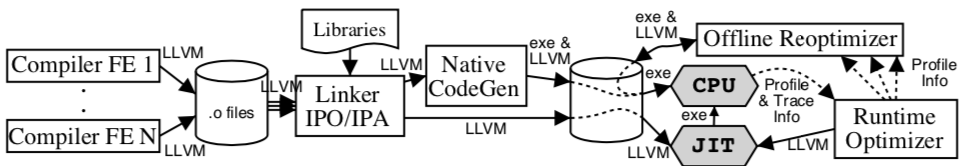
\includegraphics[width=\textwidth]{images/llvm-architecture.png}
    \caption{ The LLVM Compiler Framework Architecture \cite{lattner2004llvm}.}
    \label{fig:llvmarch}
    \Description[]{}
\end{figure*}
To achieve this ambitious goal, the framework utilizes a well defined, human-readable, intermediate representation called LLVM IR.
The IR, which is initially generated by the front end can be packaged with the target architecture binary along with profiling instructions for later runtime compilation (JIT) as well as more aggressive offline optimizations.
Several important characteristics of LLVM IR as as follows:
\begin{itemize}
    \item The IR maintains Static Single Assignment (SSA) form with unlimited virtual registers.
    \item Each register is of one of four primitive types: boolean, integer, floating-point or pointer.
    \item Similar to RISC, memory operations are carried out in registers, and between registers and memory using Load and Store instructions.
    \item The IR is limited to 31 opcodes.
    \item The IR is organized into basic blocks which must be composed into valid control flow graphs, simplifying the work required for various optimizations. 
\end{itemize}

\begin{lstlisting}[float,floatplacement=H,
caption={LLVM IR for a function multiplying x * y and adding z \cite{LLVM_Jit_Tutorial}},
label=lst:llvm_ir]
define i32 @mul_add(i32 %x, i32 %y, i32 %z) {
    entry:
    %tmp = mul i32 %x, %y
    %tmp2 = add i32 %tmp, %z
    ret i32 %tmp2
}\end{lstlisting}

This report will focus on LLVM's JIT component, which can be accessed through the MCJIT API.
The MCJIT framework provides an API thats accepts IR, generates optimized machine code, and provides a function pointer for calling the generated code.
The JIT compiler offers several levels of optimization: none, less, default, and aggressive, which correspond to O0-O3.
It should be noted that the JIT compiler by default does not perform any IR optimizations or transformations.
Instead, a developer must pass the generated IR to a Pass manager with specific optimizations.
This optimized IR can then be passed to the JIT Engine.

\section{JitBuilder}
\label{sec:jitbuilder}
JITBuilder.

\section{Methodology}
Methodology

\subsection{Results}
\label{sec:results}


\section{Related Work}
\label{sec:related-work}
Related work.






\section{Future Work}
\label{sec:future-work}
Future Work
 

\section{Summary}
\label{sec:summary}
Summary

\section{Acknowledgements}

This research was conducted within the Centre for Advanced Stu-\\dies---Atlantic, Faculty of Computer Science, University of New Brunswick. The authors are grateful for the colleagues and facilities of CAS Atlantic in supporting our research. The authors would like to acknowledge the funding support provided by the Atlantic Canada Opportunities Agency (ACOA) through the Atlantic Innovation Fund (AIF) program. Furthermore, we would also like to thank the New Brunswick Innovation Foundation for contributing to this project.

\bibliographystyle{unsrt}
\bibliography{refs}{}

\end{document}
\endinput
%%
%% End of file `paper.tex'.
